
% This LaTeX was auto-generated from MATLAB code.
% To make changes, update the MATLAB code and republish this document.

\documentclass{article}
\usepackage{graphicx}
\usepackage{color}

\usepackage{amsmath}
\usepackage{amssymb}
\usepackage{listings}
\usepackage{algorithm2e}
\usepackage{float}

\usepackage{listings}
\usepackage{geometry}
\geometry{margin=1in}
\usepackage{color}
\definecolor{light-gray}{gray}{0.95}
\lstset{numbers=right, 
                numberstyle=\tiny, 
                breaklines=true,
                backgroundcolor=\color{light-gray},
                numbersep=5pt,
                xleftmargin=.5in,
                xrightmargin=.5in} 

\sloppy
\definecolor{lightgray}{gray}{0.5}
\setlength{\parindent}{0pt}

\graphicspath{ {Assignment_1_files/} }
\begin{document}

\title{Lab 1: Basics of Image Processing}
\author{Brian Hosler \& Sarah Peachey }
\maketitle 

\abstract{Stuff about images and processing them}
\newpage
\tableofcontents


\section{Contrast Enhancement}
This section involved contrast enhancement, and a comparison
of various different techniques.
\subsection{Gamma Correction}
First, a function, \verb|Gcorrection.m|, was made, to do contrast
enhancement through gamma correction. Given a grayscale image,
and a value for gamma, the function rescales every pixel to
a value between 0 and 1. Each pixel value is then raised to
the power of gamma before being cast back to an intiger between
0 and 255. The code is shown below.

%\lstinputlisting[language=Matlab]{Gcorrection.m}
\begin{lstlisting}[language=Matlab]
function [ img_out ] = Gcorrection(img_in, gama)
%Does gamma correction using the equation:
%   new=255*(old/255)^gamma
    img_out=uint8(255*(double(img_in)/255).^gama);
end
\end{lstlisting}

\subsection{Effects of Gamma Correction}
The Gcorrection function was then used with varying gamma
arguments on the same photo to show the effects of gamma
being larger than, smaller than, and equal to, unity.
When gamma was set to 1, the mean squared error between
the original and altered image was computed, to show that
when gamma is equal to 1, every value is mapped to itself.
\begin{lstlisting}[language=Matlab]
%read in the image
pout=imread('Assignment_1_Files/pout.tif');
figure
%Plot .4 enhanced image and histogram
subplot(2,3,1)
imshow(Gcorrection(pout,.4))
title('\gamma=0.4')
subplot(2,3,4)
imhist(Gcorrection(pout,.4))

%Plot unenhanced image and histogram
subplot(2,3,2)
imshow(Gcorrection(pout,1))
title(sprintf('\\gamma=1\nMSE from original: %d',immse(pout,Gcorrection(pout,1))))
subplot(2,3,5)
imhist(Gcorrection(pout,1))

%Plot 2.1 enhanced image and histogram
subplot(2,3,3)
imshow(Gcorrection(pout,2.1))
title('\gamma=2.1')
subplot(2,3,6)
imhist(Gcorrection(pout,2.1))
\end{lstlisting}


\subsection{Histogram Equalization}
Finally, Gamma correction was compared to histogram equalization
using the photo MoonPhobos.tif. This photo has a bimodal
distribution, with a concentration of pixel values near zero,
and another near 255.
\begin{lstlisting}[language=Matlab]
%Read in new photo
moonHobos=imread('Assignment_1_Files/MoonPhobos.tif');
figure
%Plot the enhanced image
subplot(1,2,1)
imshow(Gcorrection(moonHobos,.3))
title('\gamma=.3')
subplot(1,2,2)
imshow(histeq(moonHobos,256))
title('HistEQ')

figure
%Plot histograms of the enhanced image
subplot(1,2,1)
imhist(Gcorrection(moonHobos,.3))
title('\gamma=.3')
subplot(1,2,2)
imhist(histeq(moonHobos,256))
title('HistEQ')
\end{lstlisting}

The Gcorrection function is given an input $\gamma$ less than 1,
greater than 1 and equal to one. As seen in Figure \ref{pout}, when the
$\gamma=0.4 < 1$ the picture becomes much lighter. Also, the image
histogram is shifted to higher values and it shrank in width. Meaning that
the picture has higher grey values over a smaller range. When $\gamma=1$ the
original image is shown, therefore the image histogram can be used for
reference. When $\gamma=2.1 < 1$ the image pixel values are lower but
occupy a larger range than the original image. 

\begin{figure} [H]
\centering
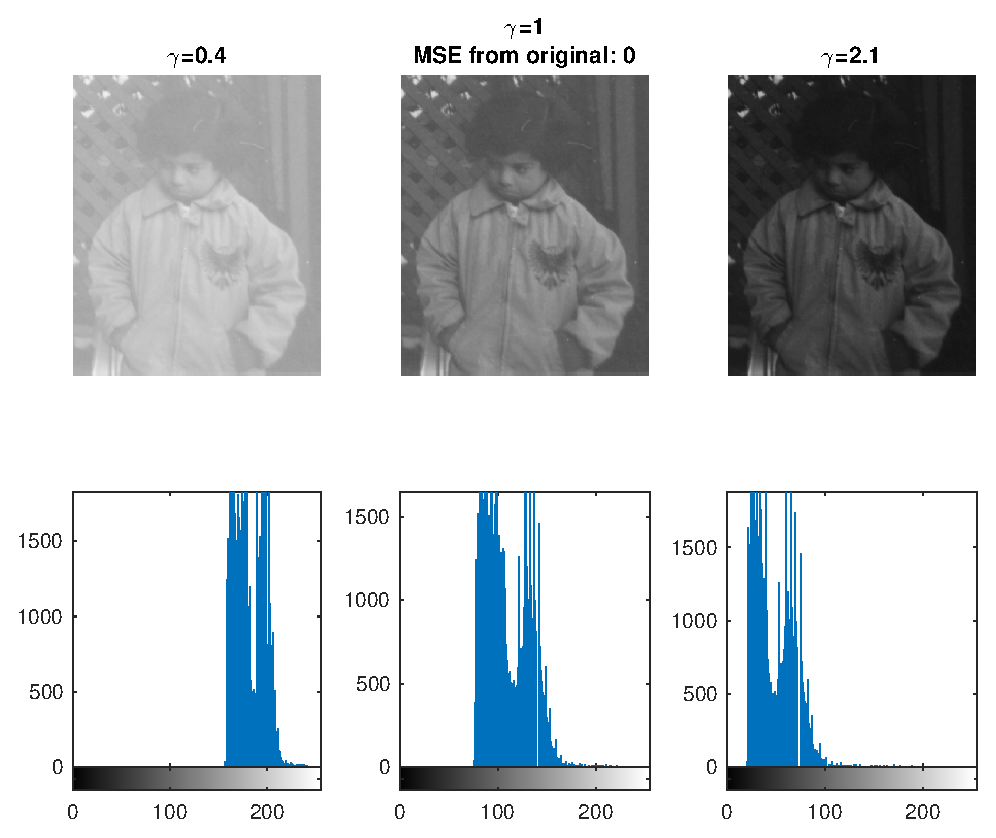
\includegraphics [width=4in]{lab1_01.eps}
\caption{Varying gamma in Gcorrection function}
\label{pout}
\end{figure}

The Gcorrection function was used to edit moonPhobos.tiff and the best
percieved version of the picture was at $\gamma=0.3$. For comparison the
MATLAB built in the function histeq was also used the results of both can be
see in \ref{MoonHobos}. As seen in \ref{moonHoboHist}, the Gcorrection
actually seemed ot spread out the values of historgram better, but by making
the pixel values lower, the image became much more dark, so some of the details
are lost. Whereas histeq does a better job of making sure the darker details
and lighter details are maintained. 


\begin{figure} [H]
\centering
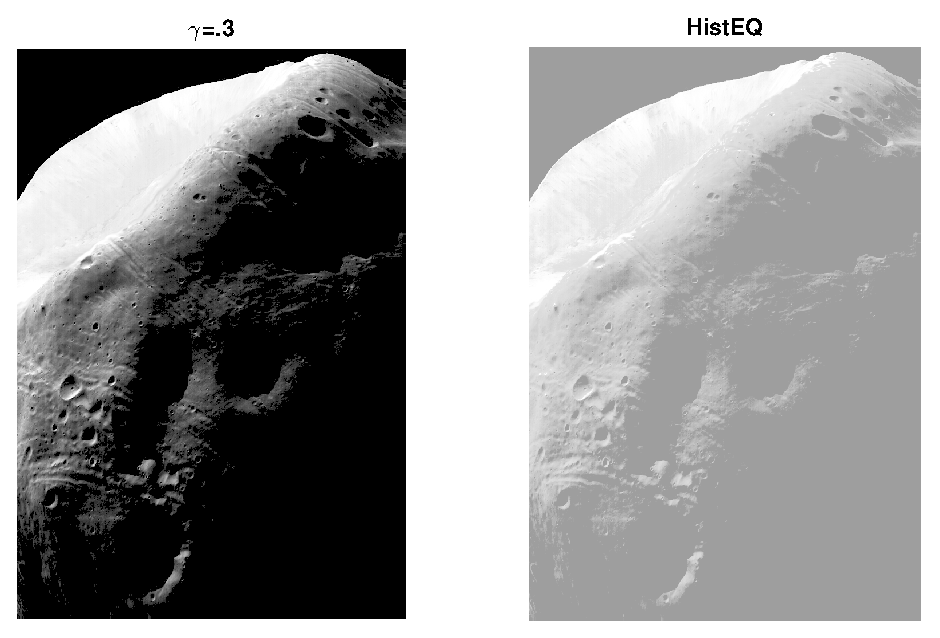
\includegraphics [width=4in]{lab1_02.eps}
\caption{Gcorrection vs Histeq}
\label{MoonHobos}
\end{figure}

\begin{figure} [H]
\centering
\includegraphics [width=4in]{lab1_03.eps}
\caption{Histograms of Gcorrection vs Histeq}
\label{moonHoboHist}
\end{figure}

\section{Part 2}

\begin{verbatim}
%1
%Our High-Boot filter function
type('HBfilt.m')

%2
%Read in and filter the moon image
moon=imread('Assignment_1_Files/moon.tiff');
figure
imshow(HBfilt(moon,2.4))
title('\alpha=2.4')

%3
%Read in a blurry image and high-boost filter it
oof=imread('Assignment_1_Files/outoffocus.tif');
figure
imshow(HBfilt(oof,4))
title('\alpha=4')
%High frequency noise added with increasing alpha(7)
\end{verbatim}

        \color{lightgray} \begin{verbatim}
function [ img_out ] = HBfilt(img_in, alph)
%High boost filtering using a laplaccian filter
    img_out=img_in+uint8(alph*conv2(double(img_in),[0 -.25 0; -.25 1 -.25; 0 -.25 0],'same'));
end

Warning: Image is too big to fit on screen; displaying at 67% 
\end{verbatim} \color{black}
    
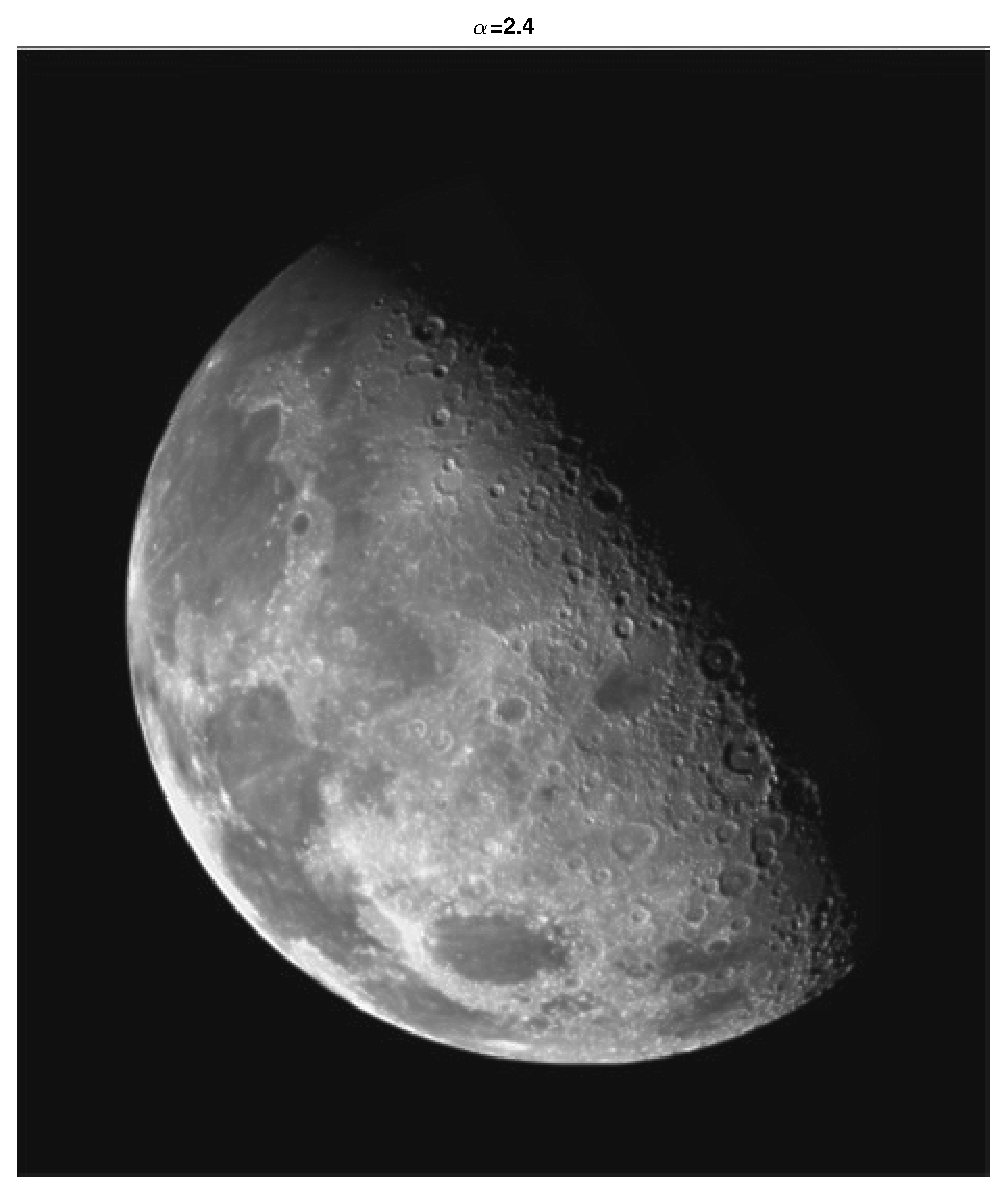
\includegraphics [width=4in]{lab1_04.eps}

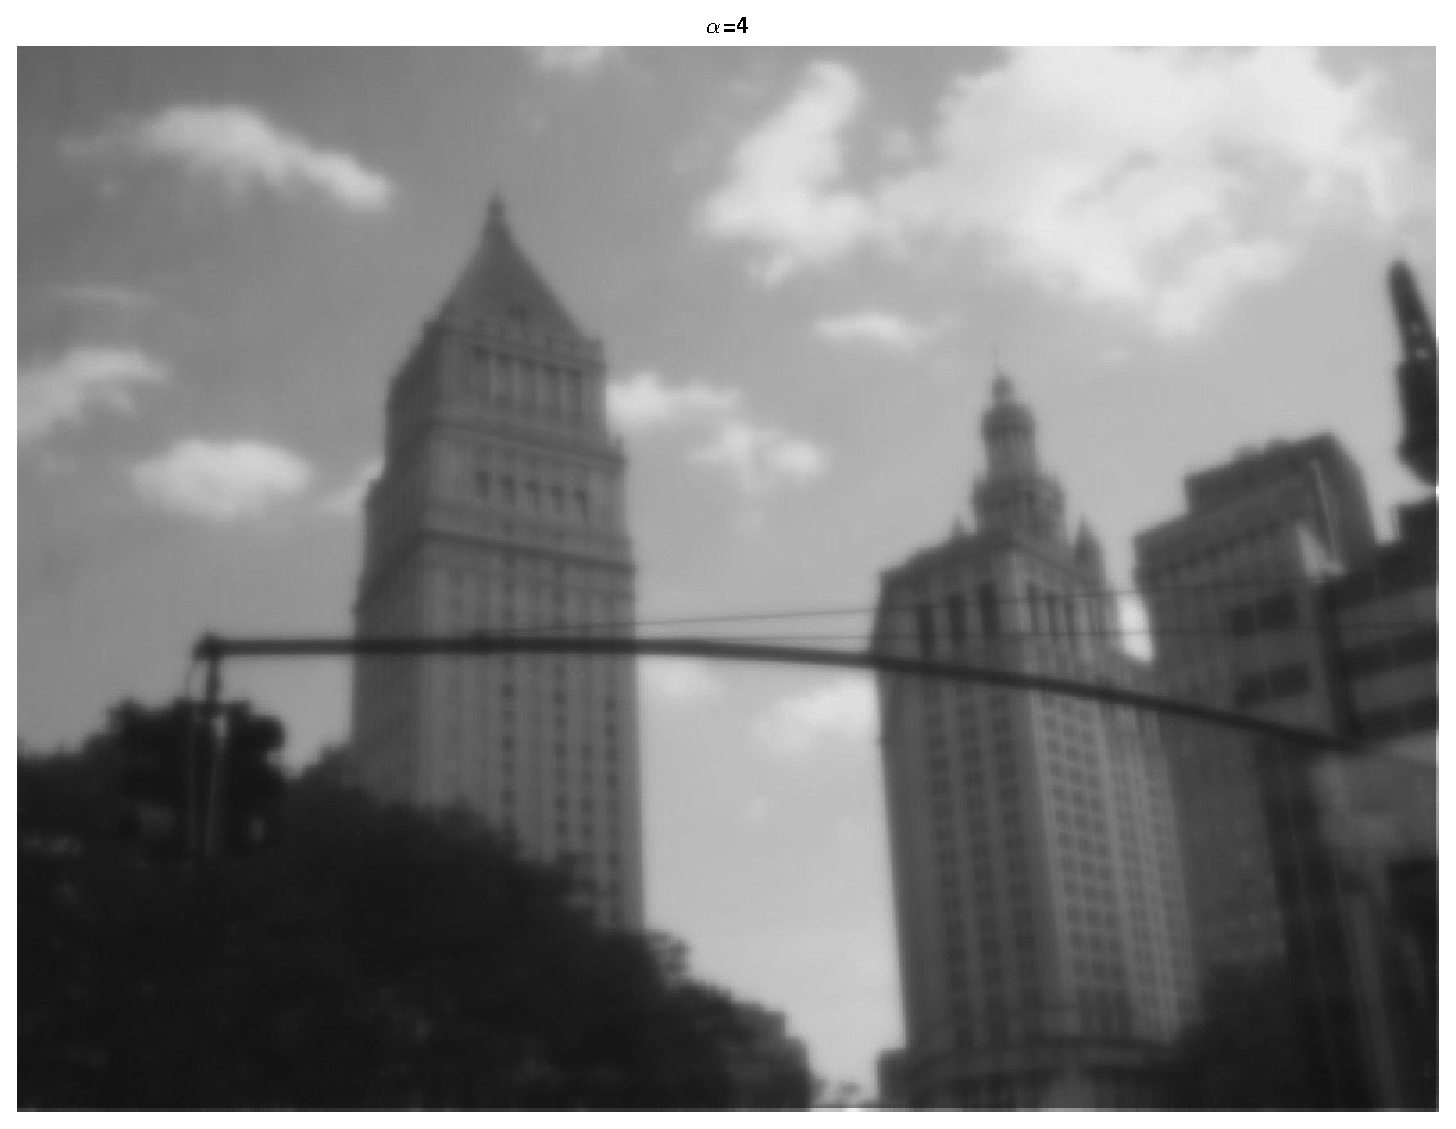
\includegraphics [width=4in]{lab1_05.eps}


\section{Part 3}

\begin{verbatim}
%1
%Read in two noidy images
pep1=imread('Assignment_1_Files/peppersNoise1.tiff');
pep2=imread('Assignment_1_Files/peppersNoise2.tiff');
figure
%Denoise images with a 3x3 median filter
subplot(4,2,1)
imshow(medfilt2(pep1,[3,3]))
title(sprintf('peppersNoise1\nMedian 3x3'))
subplot(4,2,2)
imshow(medfilt2(pep2,[3,3]))
title(sprintf('peppersNoise2\nMedian 3x3'))
%Denoise images with a 5x5 median filter
subplot(4,2,3)
imshow(medfilt2(pep1,[5,5]))
title('Median 5x5')
subplot(4,2,4)
imshow(medfilt2(pep2,[5,5]))
title('Median 5x5')
%Denoise images with a 3x3 averaging filter
subplot(4,2,5)
imshow(uint8(filter2(ones(3,3)/9,pep1)))
title('Averaging 3x3')
subplot(4,2,6)
imshow(uint8(filter2(ones(3,3)/9,pep2)))
title('Averaging 3x3')
%Denoise images with a 5x5 averaging filter
subplot(4,2,7)
imshow(uint8(filter2(ones(5,5)/25,pep1)))
title('Averaging 5x5')
subplot(4,2,8)
imshow(uint8(filter2(ones(5,5)/25,pep2)))
title('Averaging 5x5')

%2
%Save the average and median filtered images
pep1avg=uint8(filter2(ones(3,3)/9,pep1));
pep1med=medfilt2(pep1,[3,3]);
figure
th=60000;
subplot(1,2,1)
sx=filter2([-1,0,1;-2,0,2;-1,0,1],pep1avg).^2;%Xgradient
sy=filter2([-1,0,1;-2,0,2;-1,0,1].',pep1avg).^2;%Ygradient
imshow((sx+sy)>th)%Magnitude squared
subplot(1,2,2)
sx=filter2([-1,0,1;-2,0,2;-1,0,1],pep1med).^2;%Xgradient
sy=filter2([-1,0,1;-2,0,2;-1,0,1].',pep1med).^2;%Ygradient
imshow((sx+sy)>th)%Magnitude squared
\end{verbatim}

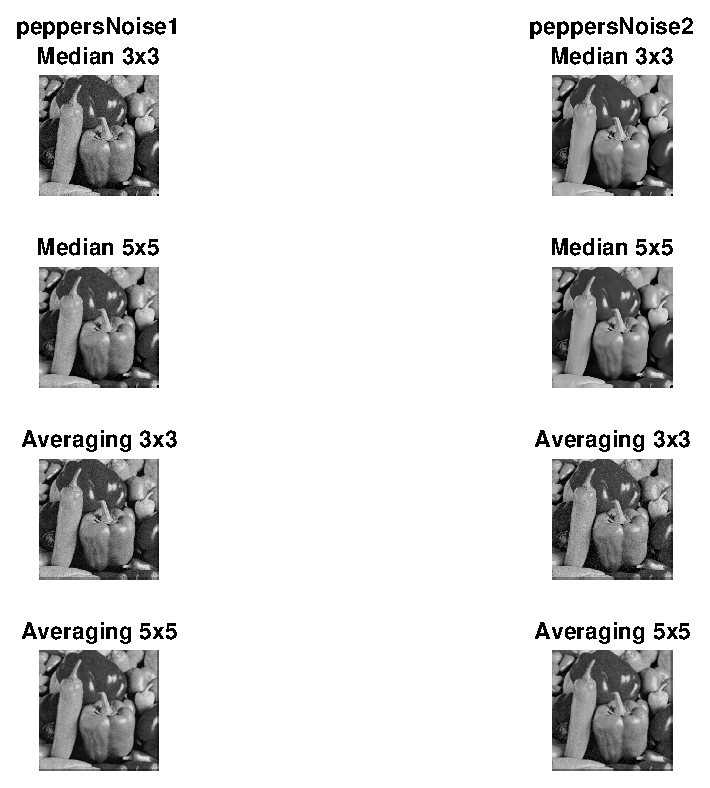
\includegraphics [width=4in]{lab1_06.eps}

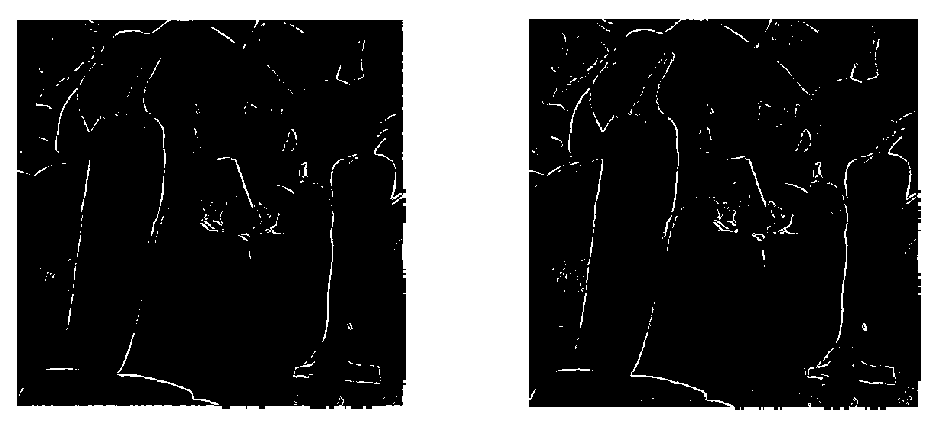
\includegraphics [width=4in]{lab1_07.eps}



\end{document}
    
